% !TEX program = xelatex
\documentclass[12pt, a4paper]{article}

\usepackage{fontspec}
\setmainfont[Ligatures=TeX]{Linux Libertine O}

\usepackage[hidelinks, colorlinks = true, urlcolor = blue]{hyperref}
\usepackage{indentfirst}
\usepackage{graphicx}
\usepackage[left=0.5cm,right=0.5cm,top=0.2cm,bottom=0.2cm]{geometry}
\usepackage{lipsum}
\usepackage{caption}
\usepackage{subcaption}
\usepackage{dirtytalk}

\usepackage{titlesec}
\titlespacing{\section}{0pc}{1.5ex plus .1ex minus .2ex}{0pc}

%\setlength{\parindent}{1em}
%\setlength{\parskip}{1em}\title{Εργασία Στατιστικής}

\title{\textbf{Parallel and Distributed Systems \\ Parallel k-Nearest Neighbors}}
\author{Θεόδωρος Κατζάλης \\ ΑΕΜ:9282 \\ katzalis@auth.gr}
\date{13/1/2020}

\begin{document}

\sloppy
%\input{titlepage}
\maketitle


%\pagebreak

\vspace{0.1cm}
\section{Introduction}
\vspace{0.2cm}

\section{Performance data}

\begin{figure}[h!]
     \begin{subfigure}[b]{0.33\textwidth}
         \centering
         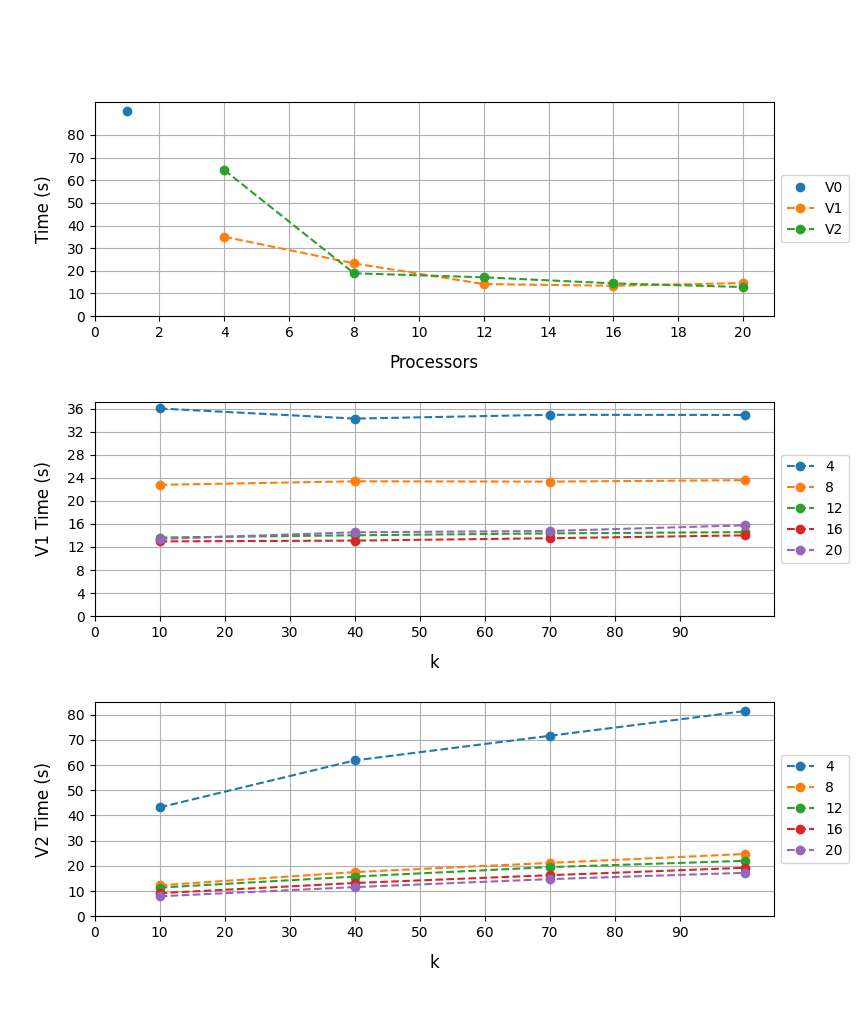
\includegraphics[height=.4\textheight, width=\textwidth, keepaspectratio]{assets/corel/histo.png}
    \caption{histo}
     \end{subfigure}
     \hfill
     \begin{subfigure}[b]{0.33\textwidth}
         \centering
         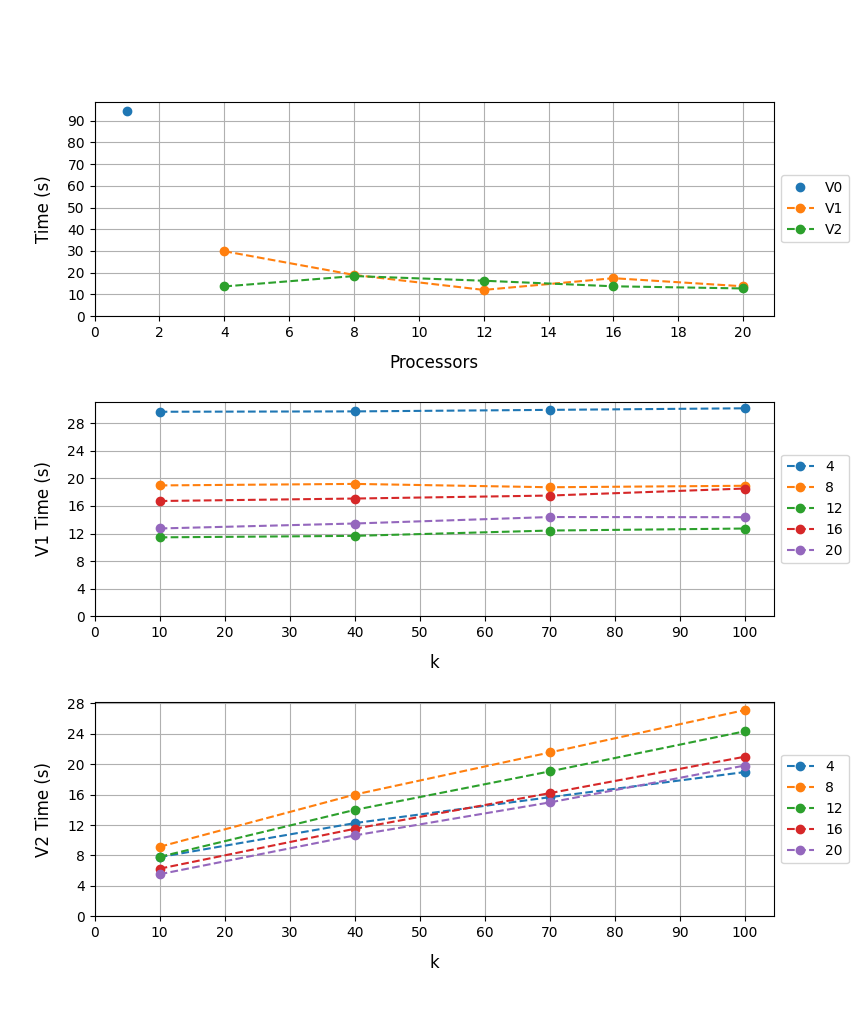
\includegraphics[height=.4\textheight, width=\textwidth, keepaspectratio]{assets/corel/moments.png}
         \caption{moments}
     \end{subfigure}
     \begin{subfigure}[b]{0.33\textwidth}
         \centering
         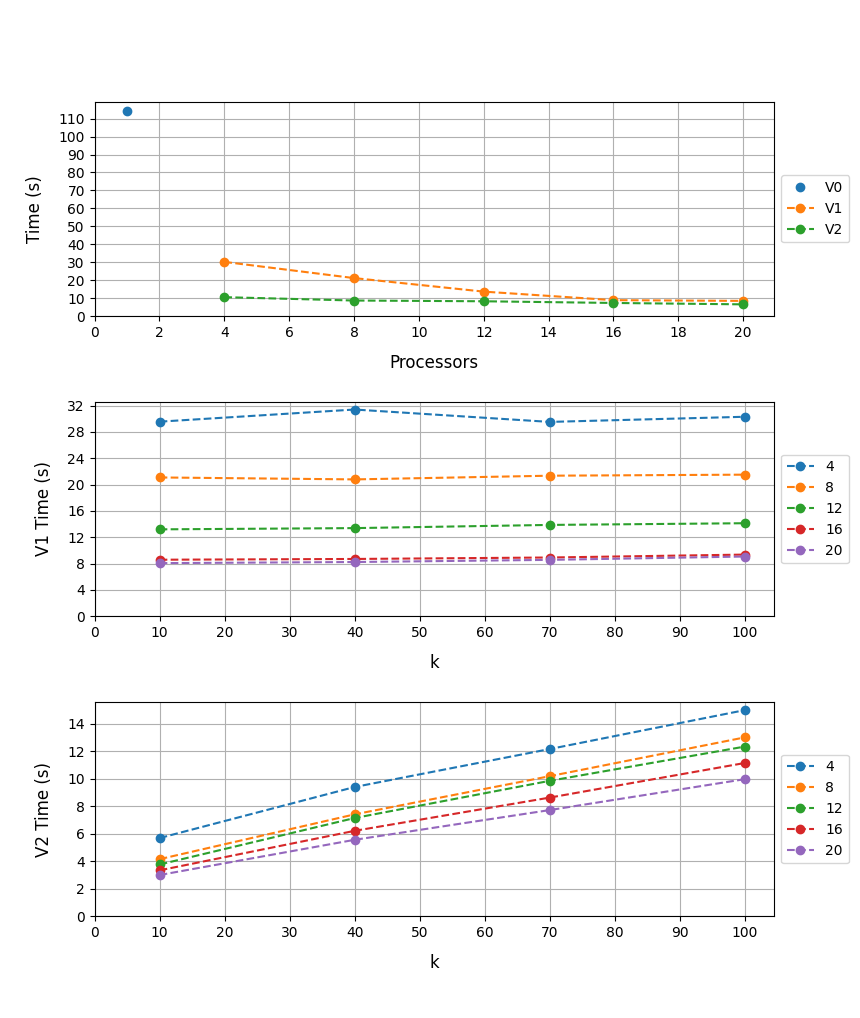
\includegraphics[height=.4\textheight, width=\textwidth, keepaspectratio]{assets/corel/texture.png}
         \caption{texture} 
     \end{subfigure}
\end{figure}


\begin{figure}[h!]
     \begin{subfigure}[b]{0.33\textwidth}
         \centering
         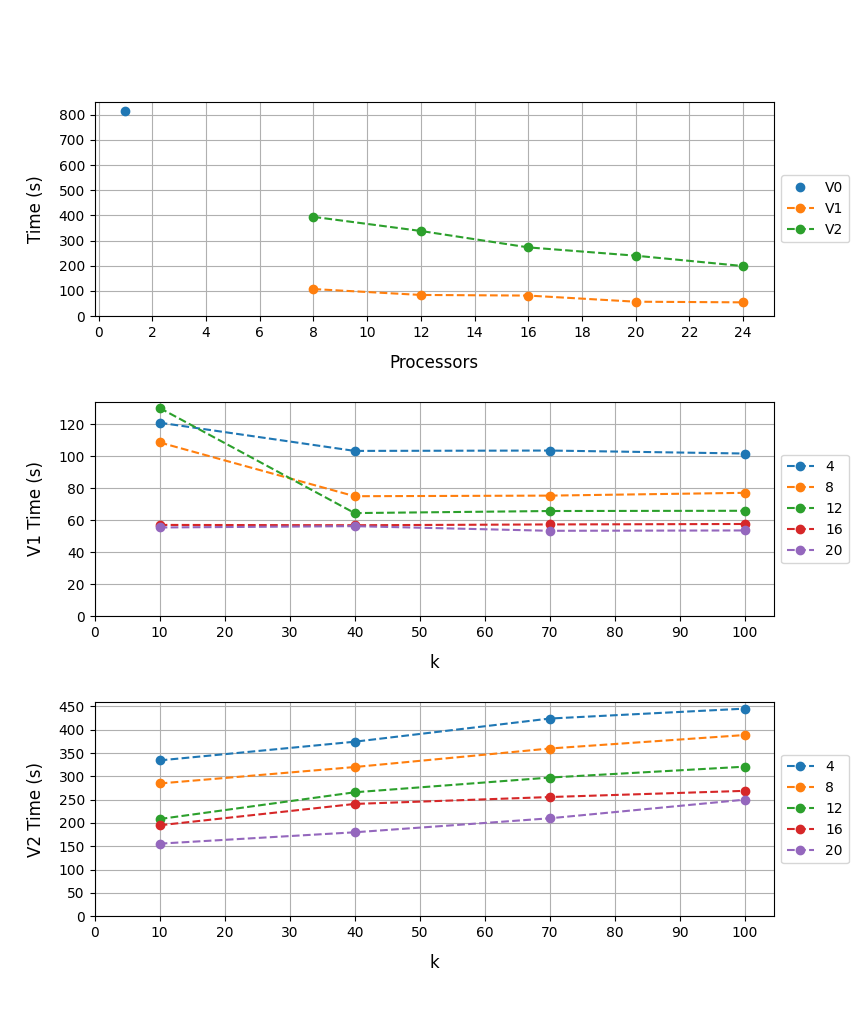
\includegraphics[height=.4\textheight, width=\textwidth, keepaspectratio]{assets/black_sheep.png}
    \caption{features}
     \end{subfigure}
     \hfill
     \begin{subfigure}[b]{0.33\textwidth}
         \centering
         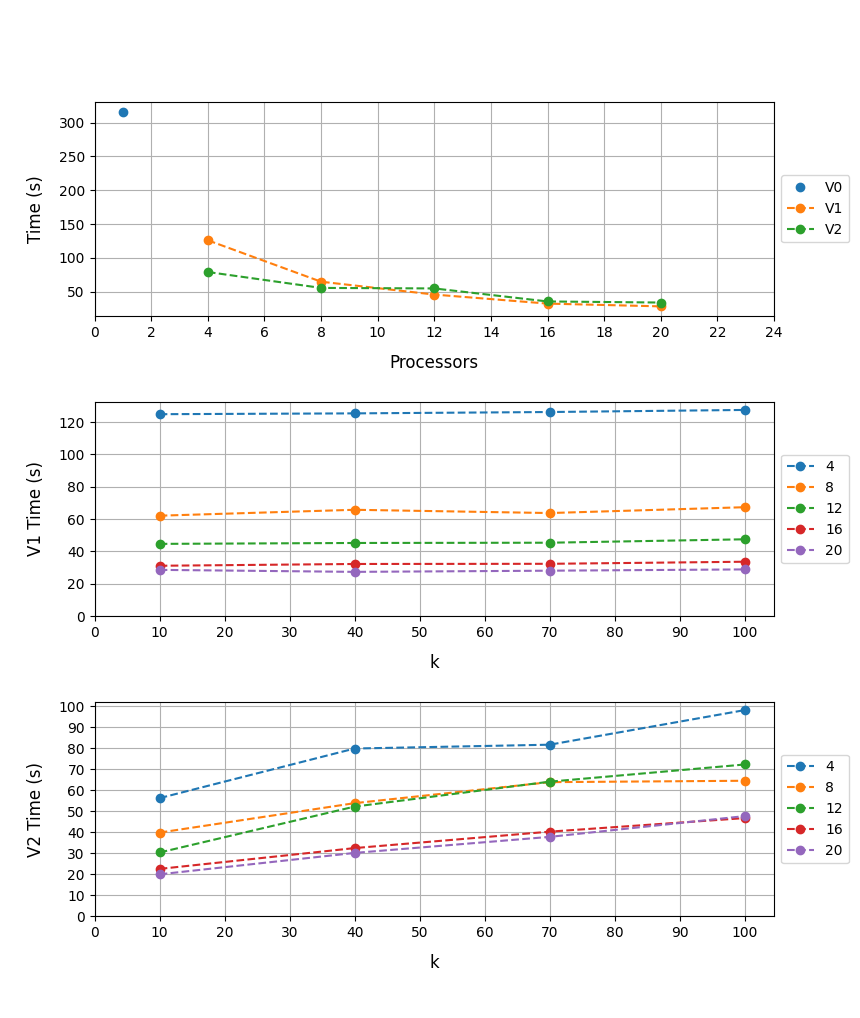
\includegraphics[height=.4\textheight, width=\textwidth, keepaspectratio]{assets/mini.png}
         \caption{mini}
     \end{subfigure}
     \begin{subfigure}[b]{0.33\textwidth}
         \centering
         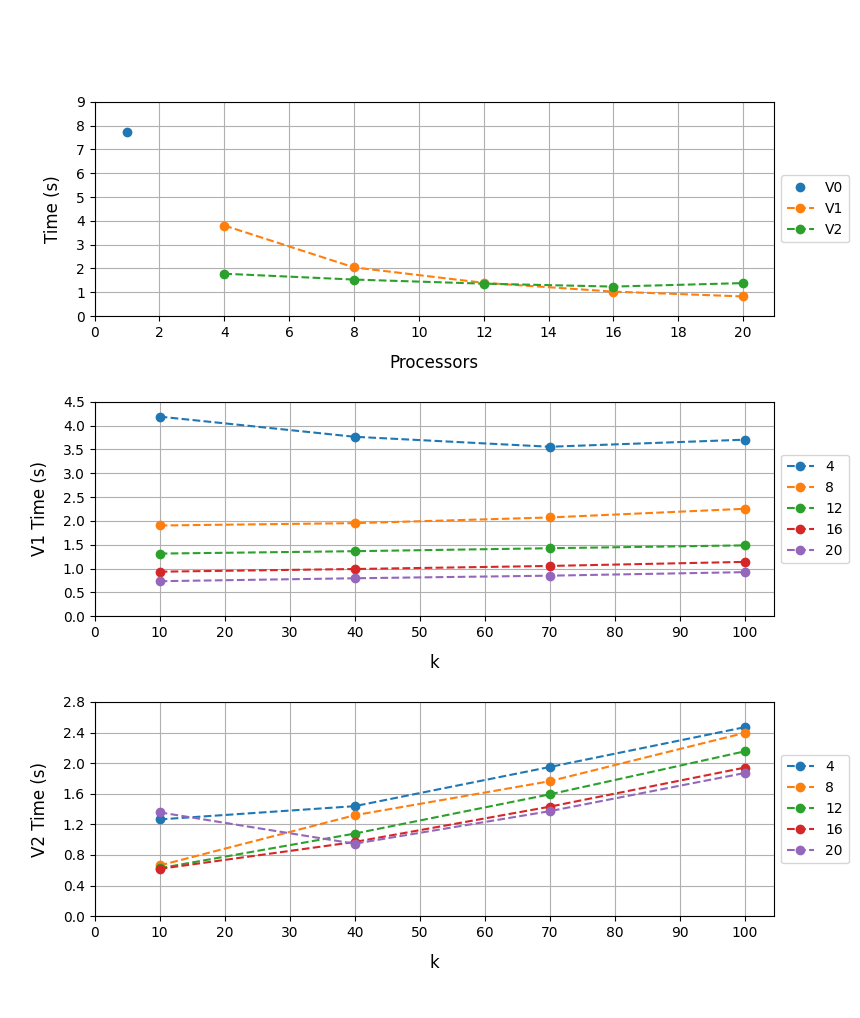
\includegraphics[height=.4\textheight, width=\textwidth, keepaspectratio]{assets/tv/bbc.png}
         \caption{bbc} 
     \end{subfigure}
\end{figure}


\begin{figure}[h!]
     \begin{subfigure}[b]{0.33\textwidth}
         \centering
         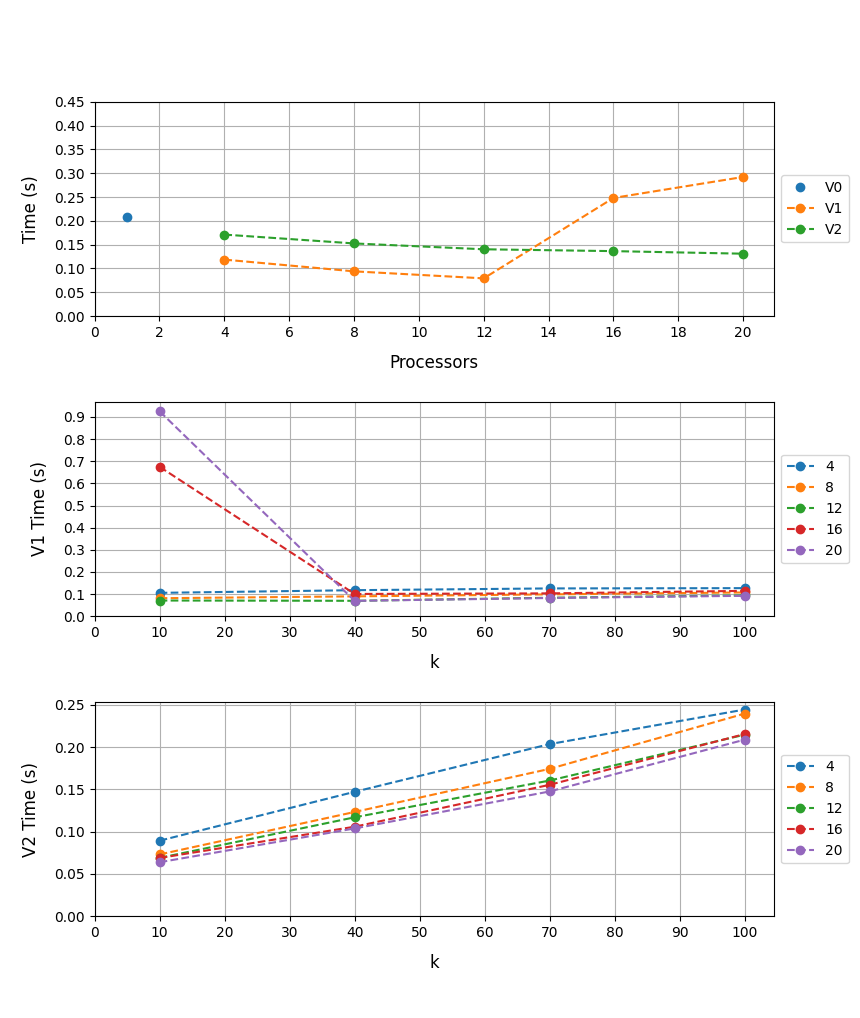
\includegraphics[height=.4\textheight, width=\textwidth, keepaspectratio]{assets/tv/cnnibn.png}
    \caption{cnnibn}
     \end{subfigure}
     \hfill
     \begin{subfigure}[b]{0.33\textwidth}
         \centering
         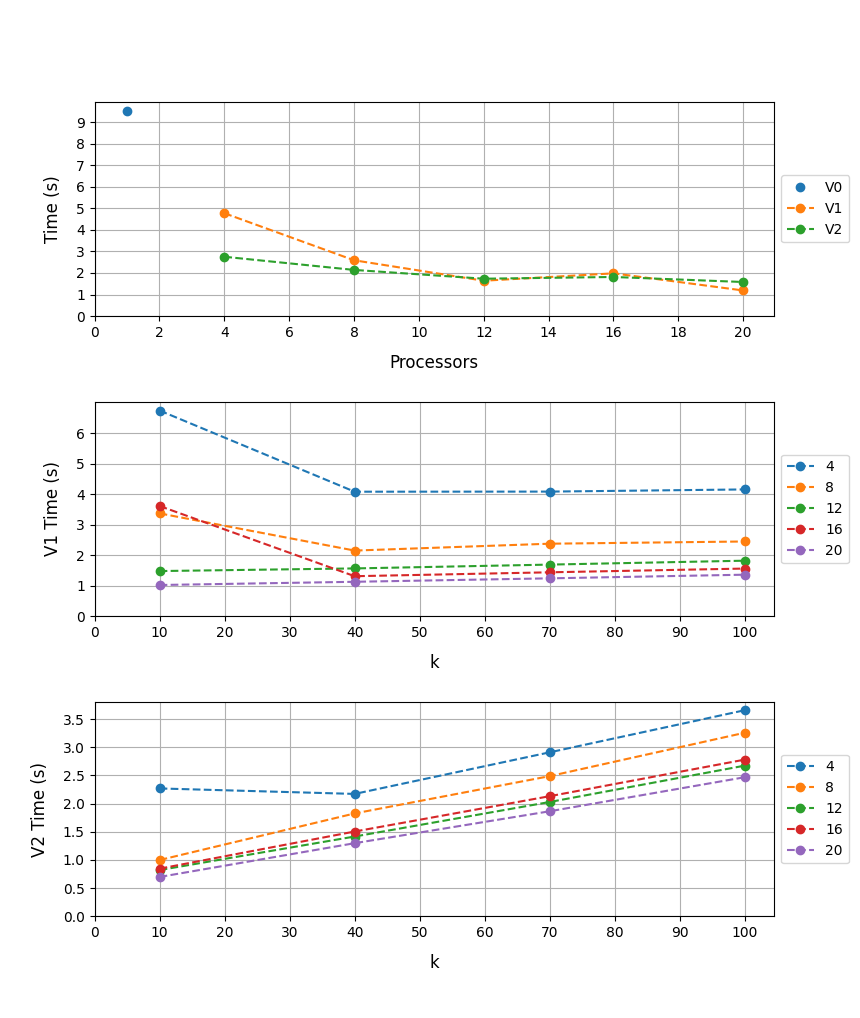
\includegraphics[height=.4\textheight, width=\textwidth, keepaspectratio]{assets/tv/cnn.png}
         \caption{cnn}
     \end{subfigure}
     \begin{subfigure}[b]{0.33\textwidth}
         \centering
         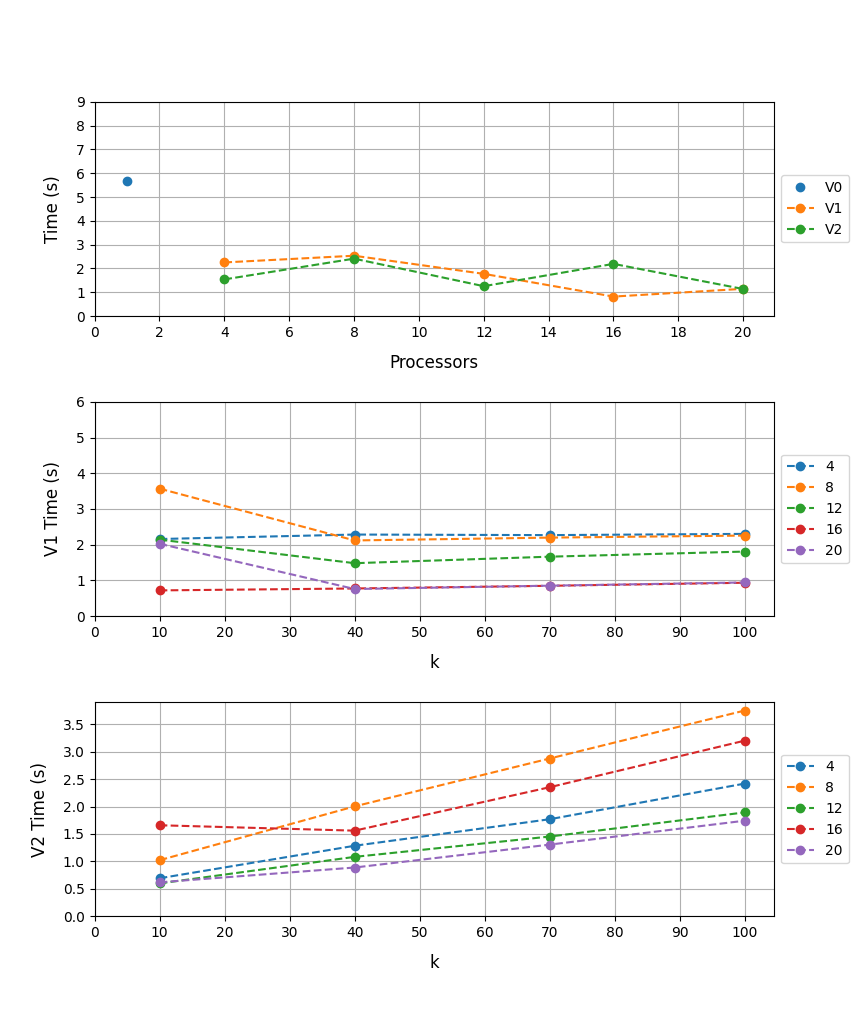
\includegraphics[height=.4\textheight, width=\textwidth, keepaspectratio]{assets/tv/ndtv.png}
         \caption{ndtv} 
     \end{subfigure}
\end{figure}

\begin{figure}[h!]
    \centering
    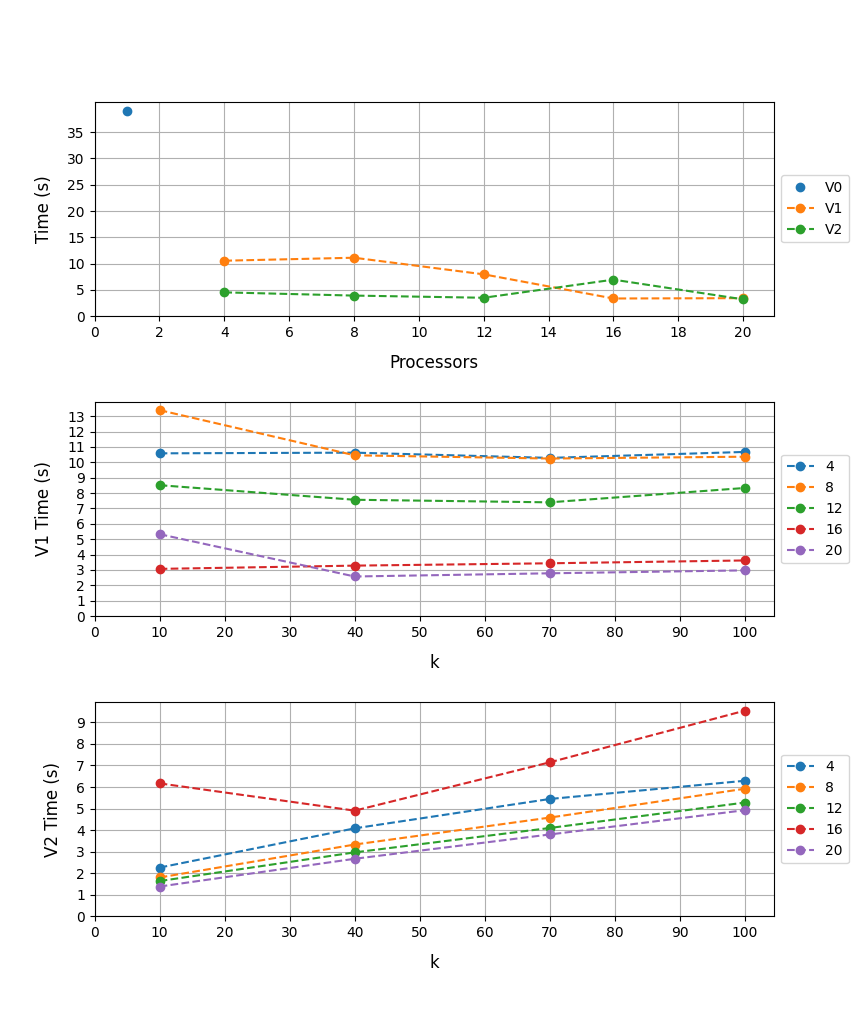
\includegraphics[height=.4\textheight, width=\textwidth, keepaspectratio]{assets/tv/timesnow.png}
    \caption{timesnow}
\end{figure}

For ccnibn. Check the twenty process performance. Cblas acceleration. The slices are too small and cblas routines are not utilised.

\end{document}
